\newpage
\section{Билет 18. Невозможность гарантированной доставки сообщений. Алгоритм скользящего окна.} \label{b18:part1}

Перейти к~\nameref{b18:part2}

\textbf{Надженость} -- доставка без потерь и дублирования. \\
A, B -- процесс, программа которая выполняется.\\
\textbf{NCP} -- Network Control Procedure, управление сетью.

У нас есть взаимодействие между приложением и NCP, между NCP и сетью передачи данных.
Между NCP и сетью передачи данных может быть протокол взаимодействия, если мы хотим обеспечить «надёжность» передачи данных (в кавычках, потому что реальную надёжность обеспечить невозможно).

Приложение А отправляет сообщение и забывает о нём, а NCP A взаимодействует с NCP B по ненадежной сети передачи данных.
У NCP есть два события: recieve \textbf{получение} -- из сети передачи данных в NCP пришло сообщение, и deliver \textbf{доставка} -- NCP решило что сообщение может быть доставлено процессу.

\newline
\begin{figure}[H] \centering
	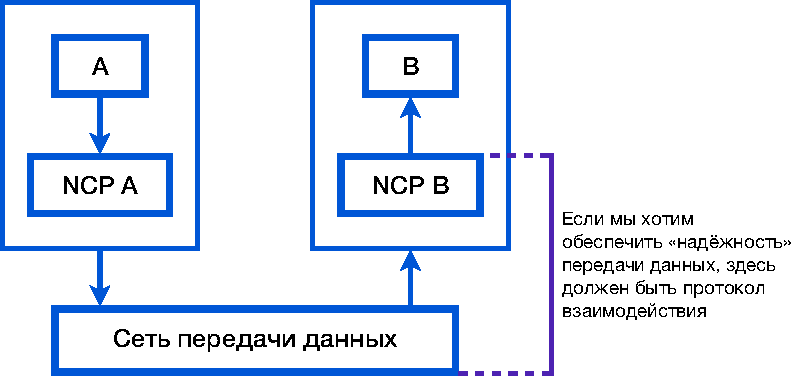
\includegraphics[scale = 1]{18/common.pdf}
\end{figure}

\textbf{Отличие recieve и deliver}: в NCP пришёл пакет 2, но не пришел пакет 1 -- событие recieve произошло, но мы не можем отправить пакет 2 в приложение, потому что нарушим порядок -- событие deliver не произошло.

Ненадженость доставки сводиться к потере пакетов в силу неисправности оборудования или ресурсного ограничения на любом шаге взаимодействия.
\bigskip

Надежная передача между А и В невозможна, например, если NCP может потерять состояние диалога (перезапуститься).
Пусть NCP B должна доставить процессу b информацию m после получения сообщения M от NCP A.
\textcolor{olive}{Здесь имеется ввиду, что B = \{процесс b + NPC B\}.}
Если NCP B перезапуститься после отправки M, то ни один из процессов не может понять было ли доставлено сообщение: у А нет информации, что происходит на стороне B (это удаленная система); так так система со стороны B перезапустилась, то она ничего не помнит.
Повторная передача может привести к дублированию, отказ -- к потере.
\textbf{Вывод: мы не можем контролировать факт доставки из NCP в процесс.}

\subsection*{Протоколы, которые передают данные между NCP.}
Рассмотрим разные жизненные протоколы общения между NCP. Их можно разделить по количеству сообщений которые передаются.

С 1 сообщением: «отправил и забыл» (UDP).

\textbf{С 2 сообщениями}: в протокол добавляется подтверждение о получении сообщения -- <\textbf{ack}> (acknowledgment).
\textcolor{olive}{\textbf{DN} (Data network) -- сеть передачи данных.}

\begin{algorithm}
	\caption{Протокол с 2 сообщениями. Нормальный сценарий.}
	\begin{enumerate}
		\item NCP A отправляет <\textbf{data}, m>
		\item NCP B получает <\textbf{data}, m> \\
			доставляет m; отправляет <\textbf{ack}>; закрывает сеанс
		\item NCP A получает <\textbf{ack}> \\
			уведомляет процесс о доставке; закрывает сеанс
	\end{enumerate}
\end{algorithm}


\begin{algorithm}
	\caption{Протокол с 2 сообщениями. Таймер. Сообщение дублируется.}
	\begin{enumerate}
		\item NCP A отправляет <\textbf{data}, m>
		\item NCP B получает <\textbf{data}, m> \\
			доставляет m; отправляет <\textbf{ack}>; закрывает сеанс
		\item DN Потеря сообщения (<\textbf{ack}>)
		\item NCP A ожидает timeout \\
			убеждается, что к нему не пришло подтверждение и отправляет <\textbf{data}, m>
		\item NCP B получает <\textbf{data}, m> \\
			доставляет m; отправляет <\textbf{ack}>; закрывает сеанс
		\item NCP A получает <\textbf{ack}> \\
			уведомляет процесс о доставке; закрывает сеанс
	\end{enumerate}
\end{algorithm}

\newpage

\textcolor{olive}{Здесь не путать сообщения протокола и те, что отправляем.}\\
В следующем примере, как и в предыдущих, протокол с 2 сообщениями (\textbf{data} + <\textbf{ack}>). И к тому же отправляем 2 сообщения <\textbf{data}, $m_1$> и <\textbf{data}, $m_2$}>.

\begin{algorithm}
	\caption{Протокол с 2 сообщениями. Потеря.}
	\begin{enumerate}
		\item NCP A отправляет <\textbf{data}, $m_1$>
		\item NCP B получает <\textbf{data}, $m_1$> \\
			доставляет $m_1$; отправляет <\textbf{ack}>; закрывает сеанс
		\item NCP A ожидает timeout \\
			убеждается, что к нему не пришло подтверждение и отправляет <\textbf{data},  $m_1$>
		\item NCP B получает <\textbf{data},  $m_1$> \\
			доставляет m; отправляет <\textbf{ack}>; закрывает сеанс
		\item NCP A получает <\textbf{ack}> (отправленное на шаге 4) \\
			уведомляет процесс о доставке; закрывает сеанс
		\item NCP A отправляет <\textbf{data}, $m_2$>
		\item DN Потеря сообщения (<\textbf{data}, $m_2$>)
		\item NCP A получает <\textbf{ack}> (отправленное на шаге 2) \\
			уведомляет процесс о доставке; закрывает сеанс
	\end{enumerate}
\end{algorithm}

Получилось, что А получил дважды подтверждение от получении <\textbf{data}, $m_1$>, но с его стороны это выглядело как 2 подтверждения для $m_1$ и $m_2$. Процесс А думает, что передача успешная, а на самом деле B не получил второе сообщение.

\newpage
\textbf{С 3 сообщениями}: в протокол хотим добавить подтверждение, что получено подтверждение <\textbf{close}>. Повторная передача при потере <\textbf{data}, m> или <\textbf{ack}>.

\begin{algorithm}
	\caption{Протокол с 3 сообщениями. Нормальный сценарий.}
	\begin{enumerate}
		\item NCP A отправляет <\textbf{data}, m>
		\item NCP B получает <\textbf{data}, m> \\
			доставляет m; отправляет <\textbf{ack}>
		\item NCP A получает <\textbf{ack}> \\
			уведомляет процесс о доставке; отправляет <\textbf{close}>; закрывает сеанс
		\item NCP B получает <\textbf{close}>; закрывает сеанс
	\end{enumerate}
\end{algorithm}

\begin{algorithm}[h!]
	\caption{Протокол с 3 сообщениями. Потеря.}
	\begin{enumerate}
		\item NCP A отправляет <\textbf{data}, $m_1$>
		\item NCP B получает <\textbf{data}, $m_1$> \\
			доставляет $m_1$; отправляет <\textbf{ack}>
		\item NCP A получает <\textbf{ack}> \\
			уведомляет процесс о доставке; отправляет <\textbf{close}>; закрывает сеанс
		\item DN потеря сообщения (<\textbf{close}>)
		\item NCP A отправляет <\textbf{data}, $m_2$>
		\item DN потеря сообщения (<\textbf{data}, $m_2$>)
		\item NCP B ожидает timeout (ждет ответа от A, после шага 2) \\
			убеждается, что к нему не пришло подтверждение  и отправляет <\textbf{ack}>
		\item NCP A получает <\textbf{ack}> \\
			уведомляет процесс о доставке; <\textbf{close}>; закрывает сеанс
		\item NCP B получает <\textbf{close}>; закрывает сеанс
	\end{enumerate}
\end{algorithm}


Получилось, что B отправил повторный <\textbf{ack}>, так как не получил от А  <\textbf{close}>. Процесс А думает, что это были 2 подтверждения на получение сообщений $m_1$ и $m_2$. Хотя на самом деле B не получил второе сообщение.

\subsection*{Алгоритм скользящего окна.}\label{b18:part2}

Перейти к~\nameref{b18:part1}

\href{https://www.youtube.com/watch?v=hd6QNXK5rPk}{Хорошее видео на эту тему.}

Раннее рассмотренные протоколы, после отправки ждут подтверждения. Скользящее окно применяется в протоколе TCP.

Концепция \textbf{скользящего окна} (sliding window) заключается в том, что для повышения скорости передачи данных отправителю разрешается передать некоторое количество сообщений, не дожидаясь прихода на эти пакеты подтверждения.

\begin{figure}[H] \centering
	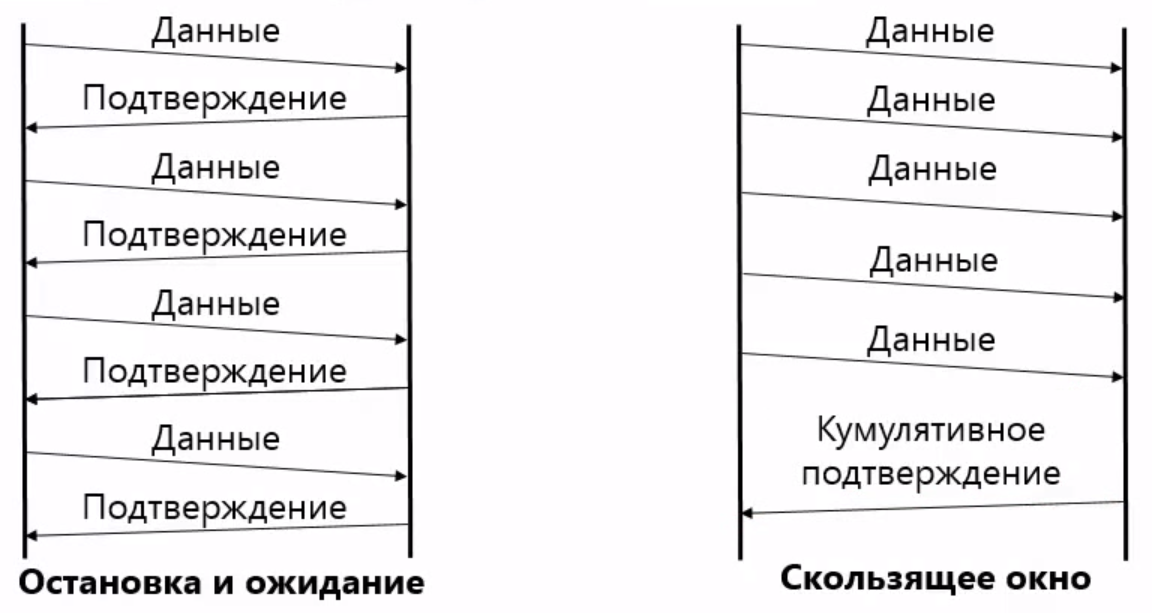
\includegraphics[scale = 0.35]{18/send_types.png}
	\caption{Схематичное различие ранее рассмотренных протоколов и алгоритма скользящего окна}
\end{figure}

\textbf{Размер скользящего окна} -- количество сообщений, которые могут быть отправлены без подтверждения. \\
В примере будет окно размера 8. Без подтверждения можем отправить 8 сообщений.
\begin{figure}[H] \centering
	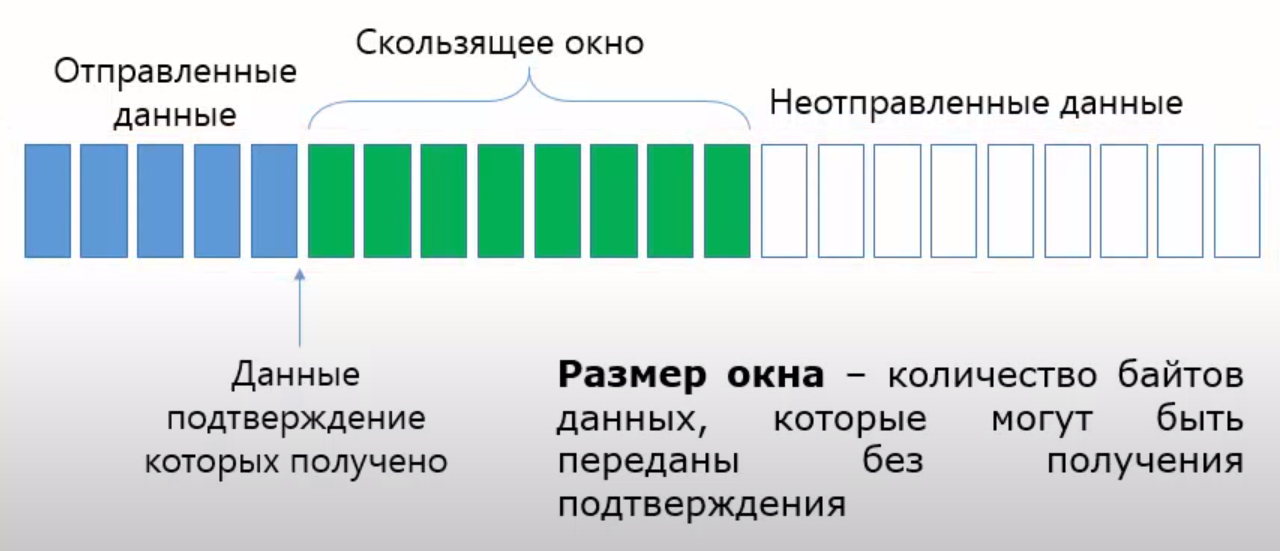
\includegraphics[scale = 0.3]{18/window_1.png}
\end{figure}

Получили часть подтверждений на ранее отправленные данные -- сдвигаем окно на количество полученных подтверждений и отправляем новую порцию данных. В примере получили 3 подтверждения, сдвинули окно на 3, отправили ещё 3 сообщения. После этого отправитель ожидает подтверждения.

\begin{figure}[H] \centering
	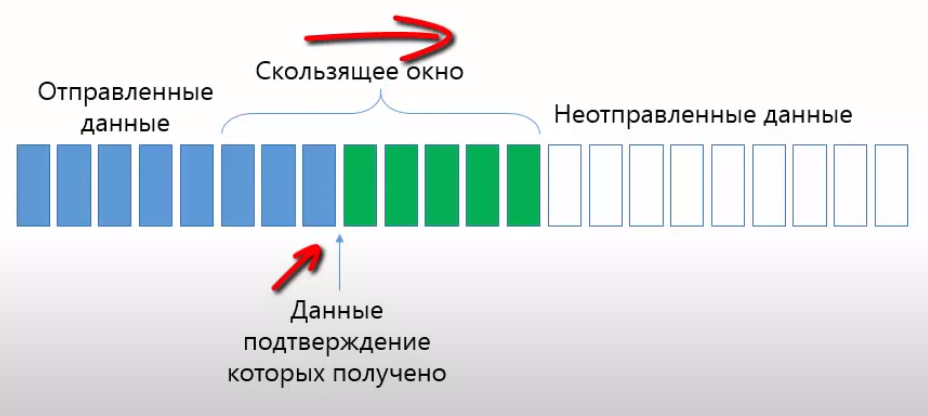
\includegraphics[scale = 0.4]{18/window_2.png}
	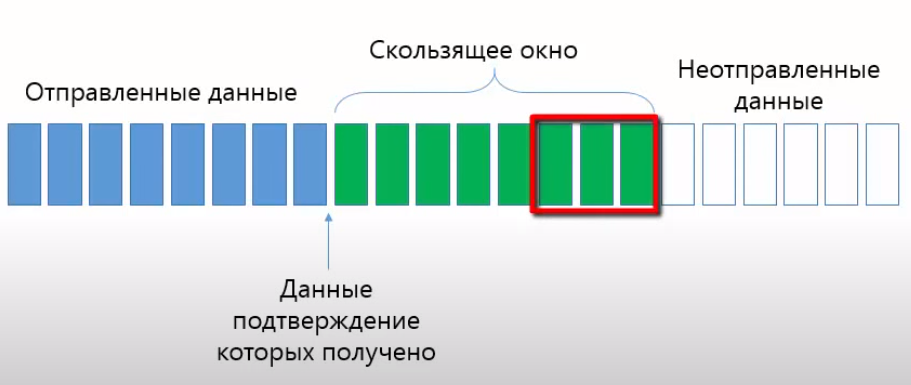
\includegraphics[scale = 0.4]{18/window_3.png}
	\caption{Сдвиг окна}
\end{figure}
